%% abtex2-modelo-trabalho-academico.tex, v-1.9.6 laurocesar
%% Copyright 2012-2016 by abnTeX2 group at http://www.abntex.net.br/ 
%%
%% This work may be distributed and/or modified under the
%% conditions of the LaTeX Project Public License, either version 1.3
%% of this license or (at your option) any later version.
%% The latest version of this license is in
%%   http://www.latex-project.org/lppl.txt
%% and version 1.3 or later is part of all distributions of LaTeX
%% version 2005/12/01 or later.
%%
%% This work has the LPPL maintenance status `maintained'.
%% 
%% The Current Maintainer of this work is the abnTeX2 team, led
%% by Lauro César Araujo. Further information are available on 
%% http://www.abntex.net.br/
%%
%% This work consists of the files abntex2-modelo-trabalho-academico.tex,
%% abntex2-modelo-include-comandos and abntex2-modelo-references.bib
%%

% ------------------------------------------------------------------------
% ------------------------------------------------------------------------
% abnTeX2: Modelo de Trabalho Academico (tese de doutorado, dissertacao de
% mestrado e trabalhos monograficos em geral) em conformidade com 
% ABNT NBR 14724:2011: Informacao e documentacao - Trabalhos academicos -
% Apresentacao
% ------------------------------------------------------------------------
% ------------------------------------------------------------------------

\documentclass[
	% -- opções da classe memoir --
	12pt,				% tamanho da fonte
	openright,			% capítulos começam em pág ímpar (insere página vazia caso preciso)
	oneside,			% para impressão em recto e verso. Oposto a oneside
	a4paper,			% tamanho do papel. 
	% -- opções da classe abntex2 --
	%chapter=TITLE,		% títulos de capítulos convertidos em letras maiúsculas
	%section=TITLE,		% títulos de seções convertidos em letras maiúsculas
	%subsection=TITLE,	% títulos de subseções convertidos em letras maiúsculas
	%subsubsection=TITLE,% títulos de subsubseções convertidos em letras maiúsculas
	% -- opções do pacote babel --
	english,			% idioma adicional para hifenização
	french,				% idioma adicional para hifenização
	spanish,			% idioma adicional para hifenização
	brazil				% o último idioma é o principal do documento
	]{abntex2}

% ---
% Pacotes básicos 
% ---
\usepackage{lmodern}			% Usa a fonte Latin Modern			
\usepackage[T1]{fontenc}		% Selecao de codigos de fonte.
\usepackage[utf8]{inputenc}		% Codificacao do documento (conversão automática dos acentos)
\usepackage{lastpage}			% Usado pela Ficha catalográfica
\usepackage{indentfirst}		% Indenta o primeiro parágrafo de cada seção.
\usepackage{color}				% Controle das cores
\usepackage{graphicx}			% Inclusão de gráficos
\usepackage{microtype} 			% para melhorias de justificação
% ---
		
% ---
% Pacotes adicionais, usados apenas no âmbito do Modelo Canônico do abnteX2
% ---
\usepackage{lipsum}				% para geração de dummy text
% ---

% ---
% Pacotes de citações
% ---
%\usepackage[brazilian,hyperpageref]{backref}	 % Paginas com as citações na bibl
\usepackage[alf]{abntex2cite}	% Citações padrão ABNT

% --- 
% CONFIGURAÇÕES DE PACOTES
% --- 

% ---
% Configurações do pacote backref
% Usado sem a opção hyperpageref de backref
%\renewcommand{\backrefpagesname}{Citado na(s) página(s):~}
%% Texto padrão antes do número das páginas
%\renewcommand{\backref}{}
%% Define os textos da citação
%\renewcommand*{\backrefalt}[4]{
%	\ifcase #1 %
%		Nenhuma citação no texto.%
%	\or
%		Citado na página #2.%
%	\else
%		Citado #1 vezes nas páginas #2.%
%	\fi}%
% ---

% ---
% Informações de dados para CAPA e FOLHA DE ROSTO
% ---
\titulo{Ouve Fácil - Um aplicativo para identificação de problemas de infraestrutura, saúde e segurança em uma cidade}
\autor{Matheus Mauricio de Souza Araujo}
\local{Cachoeiro de Itapemirim}
\data{2016, v-1.2}
\orientador{Flávio Izo}
\instituicao{%
  Instituto Federal de Educação, Ciência e Tecnologia do Espírito Santo -- Ifes
  \par
  Curso de Bacharelado em Sistemas de Informação
  \par
  Anteprojeto de Trabalho de Conclusão do Curso Bacharelado em Sistemas de Informação }
\tipotrabalho{Trabalho de Conclusão de Curso}
% O preambulo deve conter o tipo do trabalho, o objetivo, 
% o nome da instituição e a área de concentração 
\preambulo{Anteprojeto apresentado na Disciplina de Anteprojeto do Curso Bacharelado em Sistemas de Informação como requisito parcial da disciplina.}
% ---


% ---
% Configurações de aparência do PDF final

% alterando o aspecto da cor azul
\definecolor{blue}{RGB}{41,5,195}

% informações do PDF
\makeatletter
\hypersetup{
     	%pagebackref=true,
		pdftitle={\@title}, 
		pdfauthor={\@author},
    	pdfsubject={\imprimirpreambulo},
	    pdfcreator={TCC},
		pdfkeywords={Aplicação}{cidade}{problemas}{\textit{crowdsourcing}}, 
		colorlinks=true,       		% false: boxed links; true: colored links
    	linkcolor=black,          	% color of internal links
    	citecolor=black,        		% color of links to bibliography
    	filecolor=black,      		% color of file links
		urlcolor=black,
		bookmarksdepth=4
}
\makeatother
% --- 

% --- 
% Espaçamentos entre linhas e parágrafos 
% --- 

% O tamanho do parágrafo é dado por:
\setlength{\parindent}{1.3cm}

% Controle do espaçamento entre um parágrafo e outro:
\setlength{\parskip}{0.2cm}  % tente também \onelineskip

% ---
% compila o indice
% ---
\makeindex
% ---

% ----
% Início do documento
% ----
\begin{document}

% Seleciona o idioma do documento (conforme pacotes do babel)
%\selectlanguage{english}
\selectlanguage{brazil}

% Retira espaço extra obsoleto entre as frases.
\frenchspacing 

% ----------------------------------------------------------
% ELEMENTOS PRÉ-TEXTUAIS
% ----------------------------------------------------------
% \pretextual

% ---
% Capa
% ---
\imprimircapa
% ---

% ---
% Folha de rosto
% (o * indica que haverá a ficha bibliográfica)
% ---
\imprimirfolhaderosto*
% ---

% ---
% Inserir a ficha bibliografica
% ---

% Isto é um exemplo de Ficha Catalográfica, ou ``Dados internacionais de
% catalogação-na-publicação''. Você pode utilizar este modelo como referência. 
% Porém, provavelmente a biblioteca da sua universidade lhe fornecerá um PDF
% com a ficha catalográfica definitiva após a defesa do trabalho. Quando estiver
% com o documento, salve-o como PDF no diretório do seu projeto e substitua todo
% o conteúdo de implementação deste arquivo pelo comando abaixo:
%
% \begin{fichacatalografica}
%     \includepdf{fig_ficha_catalografica.pdf}
% \end{fichacatalografica}

%\begin{fichacatalografica}
%	\sffamily
%	\vspace*{\fill}					% Posição vertical
%	\begin{center}					% Minipage Centralizado
%	\fbox{\begin{minipage}[c][8cm]{13.5cm}		% Largura
%	\small
%	\imprimirautor
%	%Sobrenome, Nome do autor
%	
%	\hspace{0.5cm} \imprimirtitulo  / \imprimirautor. --
%	\imprimirlocal, \imprimirdata-
%	
%	\hspace{0.5cm} \pageref{LastPage} p. : il. (algumas color.) ; 30 cm.\\
%	
%	\hspace{0.5cm} \imprimirorientadorRotulo~\imprimirorientador\\
%	
%	\hspace{0.5cm}
%	\parbox[t]{\textwidth}{\imprimirtipotrabalho~--~\imprimirinstituicao,
%	\imprimirdata.}\\
%	
%	\hspace{0.5cm}
%		1. Palavra-chave1.
%		2. Palavra-chave2.
%		2. Palavra-chave3.
%		I. Orientador.
%		II. Universidade xxx.
%		III. Faculdade de xxx.
%		IV. Título 			
%	\end{minipage}}
%	\end{center}
%\end{fichacatalografica}
% ---

% ---
% Inserir errata
% ---
%\begin{errata}
%Elemento opcional da \citeonline[4.2.1.2]{NBR14724:2011}. Exemplo:
%
%\vspace{\onelineskip}
%
%FERRIGNO, C. R. A. \textbf{Tratamento de neoplasias ósseas apendiculares com
%reimplantação de enxerto ósseo autólogo autoclavado associado ao plasma
%rico em plaquetas}: estudo crítico na cirurgia de preservação de membro em
%cães. 2011. 128 f. Tese (Livre-Docência) - Faculdade de Medicina Veterinária e
%Zootecnia, Universidade de São Paulo, São Paulo, 2011.
%
%\begin{table}[htb]
%\center
%\footnotesize
%\begin{tabular}{|p{1.4cm}|p{1cm}|p{3cm}|p{3cm}|}
%  \hline
%   \textbf{Folha} & \textbf{Linha}  & \textbf{Onde se lê}  & \textbf{Leia-se}  \\
%    \hline
%    1 & 10 & auto-conclavo & autoconclavo\\
%   \hline
%\end{tabular}
%\end{table}
%
%\end{errata}
% ---

% ---
% Inserir folha de aprovação
% ---

% Isto é um exemplo de Folha de aprovação, elemento obrigatório da NBR
% 14724/2011 (seção 4.2.1.3). Você pode utilizar este modelo até a aprovação
% do trabalho. Após isso, substitua todo o conteúdo deste arquivo por uma
% imagem da página assinada pela banca com o comando abaixo:
%
% \includepdf{folhadeaprovacao_final.pdf}
%
%\begin{folhadeaprovacao}
%
%  \begin{center}
%    {\ABNTEXchapterfont\large\imprimirautor}
%
%    \vspace*{\fill}\vspace*{\fill}
%    \begin{center}
%      \ABNTEXchapterfont\bfseries\Large\imprimirtitulo
%    \end{center}
%    \vspace*{\fill}
%    
%    \hspace{.45\textwidth}
%    \begin{minipage}{.5\textwidth}
%        \imprimirpreambulo
%    \end{minipage}%
%    \vspace*{\fill}
%   \end{center}
%        
%   Trabalho aprovado. \imprimirlocal, 24 de novembro de 2012:
%
%   \assinatura{\textbf{\imprimirorientador} \\ Orientador} 
%   \assinatura{\textbf{Professor} \\ Convidado 1}
%   \assinatura{\textbf{Professor} \\ Convidado 2}
%   %\assinatura{\textbf{Professor} \\ Convidado 3}
%   %\assinatura{\textbf{Professor} \\ Convidado 4}
%      
%   \begin{center}
%    \vspace*{0.5cm}
%    {\large\imprimirlocal}
%    \par
%    {\large\imprimirdata}
%    \vspace*{1cm}
%  \end{center}
%  
%\end{folhadeaprovacao}
% ---

% ---
% Dedicatória
%% ---
%\begin{dedicatoria}
%   \vspace*{\fill}
%   \centering
%   \noindent
%   \textit{ Este trabalho é dedicado às crianças adultas que,\\
%   quando pequenas, sonharam em se tornar cientistas.} \vspace*{\fill}
%\end{dedicatoria}
%% ---
%
%% ---
%% Agradecimentos
%% ---
%\begin{agradecimentos}
%Os agradecimentos principais são direcionados à Gerald Weber, Miguel Frasson,
%Leslie H. Watter, Bruno Parente Lima, Flávio de Vasconcellos Corrêa, Otavio Real
%Salvador, Renato Machnievscz\footnote{Os nomes dos integrantes do primeiro
%projeto abn\TeX\ foram extraídos de
%\url{http://codigolivre.org.br/projects/abntex/}} e todos aqueles que
%contribuíram para que a produção de trabalhos acadêmicos conforme
%as normas ABNT com \LaTeX\ fosse possível.
%
%Agradecimentos especiais são direcionados ao Centro de Pesquisa em Arquitetura
%da Informação\footnote{\url{http://www.cpai.unb.br/}} da Universidade de
%Brasília (CPAI), ao grupo de usuários
%\emph{latex-br}\footnote{\url{http://groups.google.com/group/latex-br}} e aos
%novos voluntários do grupo
%\emph{\abnTeX}\footnote{\url{http://groups.google.com/group/abntex2} e
%\url{http://www.abntex.net.br/}}~que contribuíram e que ainda
%contribuirão para a evolução do \abnTeX.
%
%\end{agradecimentos}
%% ---
%
%% ---
%% Epígrafe
%% ---
%\begin{epigrafe}
%    \vspace*{\fill}
%	\begin{flushright}
%		\textit{``Não vos amoldeis às estruturas deste mundo, \\
%		mas transformai-vos pela renovação da mente, \\
%		a fim de distinguir qual é a vontade de Deus: \\
%		o que é bom, o que Lhe é agradável, o que é perfeito.\\
%		(Bíblia Sagrada, Romanos 12, 2)}
%	\end{flushright}
%\end{epigrafe}
% ---

% resumo em português
\setlength{\absparsep}{18pt} % ajusta o espaçamento dos parágrafos do resumo
\begin{resumo}
 Dentro de uma cidade, existem diversos problemas de infraestrutura, segurança e saúde que afetam a população. Identificar, analisar e resolver esses problemas demanda muito tempo, gastos e atenção dos órgãos responsáveis por realizar essa fiscalização. Tais recursos poderiam ser minimizados com a ajuda dos cidadãos a partir de um sistema informatizado, além do tradicional telefone para contato.
 \\Esse trabalho tem como finalidade a criação de uma aplicação para dispositivos móveis com sistema operacional Android, a qual seria capaz de alertar os cidadãos, através de fotografias anexadas a um mapa da cidade, dos problemas identificados pelos mesmos. Tais fotografias ficarão disponíveis até o momento que o órgão responsável resolva o problema e marque como corrigido na aplicação. Enquanto não é corrigido, outros usuários podem marcar o problema como “existe” ou “não existe”, confirmando ou não a autenticidade do problema.
 \\Essa participação dos usuários é considerada uma forma de \textit{crowdsourcing}, ou seja, através de uma ação conjunta dos cidadãos é possível garantir se existe ou não um problema em determinada marcação do mapa, sem a necessidade de ter um especialista naquela região. 
 
 
 \vspace{\onelineskip}
 
 \noindent
 \textbf{Palavras-chave}: Aplicação, problemas, cidade, \textit{crowdsourcing}.

\end{resumo}

% resumo em inglês
%\begin{resumo}[Abstract]
% \begin{otherlanguage*}{english}
%   This is the english abstract.
%
%   \vspace{\onelineskip}
% 
%   \noindent 
%   \textbf{Keywords}: latex. abntex. text editoration.
% \end{otherlanguage*}
%\end{resumo}
%

% inserir lista de ilustrações
%% ---
%\pdfbookmark[0]{\listfigurename}{lof}
%\listoffigures*
%\cleardoublepage
%% ---
%
%% ---
%% inserir lista de tabelas
%% ---
%\pdfbookmark[0]{\listtablename}{lot}
%\listoftables*
%\cleardoublepage
%% ---
%
%% ---
%% inserir lista de abreviaturas e siglas
%% ---
%\begin{siglas}
%  \item[ABNT] Associação Brasileira de Normas Técnicas
%  \item[abnTeX] ABsurdas Normas para TeX
%\end{siglas}
%% ---
%
%% ---
%% inserir lista de símbolos
%% ---
%\begin{simbolos}
%  \item[$ \Gamma $] Letra grega Gama
%  \item[$ \Lambda $] Lambda
%  \item[$ \zeta $] Letra grega minúscula zeta
%  \item[$ \in $] Pertence
%\end{simbolos}
%% ---
%
%% ---
%% inserir o sumario
%% ---
\pdfbookmark[0]{\contentsname}{toc}
\tableofcontents*
\cleardoublepage
%% ---
%
%
%
%% ----------------------------------------------------------
%% ELEMENTOS TEXTUAIS
%% ----------------------------------------------------------
%\textual
%
%% ----------------------------------------------------------
%%Introdução (exemplo de capítulo sem numeração, mas presente %%no Sumário)
%% ----------------------------------------------------------

\chapter[Motivação]{Motivação}

Existem situações que afetam a vida do cidadão e que estão fora de seu alcance resolver: o carro passa por cima de um buraco e quebra alguma peça, o engarrafamento está pior que o de costume devido a algum semáforo com mau funcionamento, a epidemia de dengue aumenta porquê não houve as devidas medidas de prevenção, e os entulhos jogados nas calçadas estão ficando cada vez maiores. Infelizmente esses e outros problemas de serviços urbanos são de responsabilidade da Prefeitura Municipal fiscalizar e corrigir, não estando ao alcance do cidadão a capacidade de resolvê-los, mesmo sendo o principal afetado.

Mesmo com esses e outros problemas afetando sua vida diária, geralmente não é comum os cidadãos denunciarem à Ouvidoria Pública - órgão da Prefeitura Municipal responsável por realizar tal tarefa - pelo fato de não quererem "perder" um tempo no telefone descrevendo o problema, onde ele está, quando aconteceu, entre outras perguntas, ou pelo fato de não lembrarem do problema quando chegam em casa.

Por quê usar somente os meios tradicionais, como telefone ou registrar a queixa presencialmente, quando se pode facilitar o processo e fazer uma rápida e informatizada forma de denúncia? Uma maneira de agilizar o processo de identificação e denúncia do problema, é a criação de um aplicativo para Android que será capaz de categorizar e marcar o problema a partir de uma fotografia, e marcá-lo em um mapa da cidade.

Será que com o uso desse aplicativo, a quantidade de reclamações à Ouvidoria e a quantidade de problemas resolvidos iria aumentar?

\chapter[Justificativa]{Justificativa}

Segundo \cite{polidori2005crescimento}, devido ao crescimento urbano ocorrem modificações na cidade de aspecto à paisagem, à morfologia urbana e da ecologia da paisagem. Devido a essas modificações, começam a surgir alguns problemas de serviços urbanos que antes não eram tão frequentes. Por causa desse aumento na quantidade de problemas, surge a necessidade de aprimoramento da relação da Prefeitura Municipal com os cidadãos. 

O Ouve Fácil é um aplicativo para Android que será capaz de realizar e registrar fotografias, capturar a posição global do smartphone no momento da foto (através do \textit{GPS}\footnote{GPS - Global Positioning System, traduzido para o português como Sistema de Posicionamento Global é um sistema de posicionamento por satélite que fornece a um aparelho receptor móvel sua posição e informação horária sob quaisquer condições atmosféricas}) e juntamento com uma breve descrição e categorização do problema, marcá-lo em um mapa da cidade, o qual deve conter todas as marcações que os outros usuários realizarem.

A partir do uso do aplicativo, espera-se que o período de identificação e correção do problema seja reduzido, gerando como consequência uma melhor qualidade de vida aos cidadãos, devido ao menor tempo de exposição dos munícipes ao problema, e gerando também uma forma de economizar os gastos e recursos da Prefeitura. Tais “gastos à cidade, que poderiam ser minimizados se os cidadãos pudessem identificar com antecedência – com o auxílio de sistemas informatizados – a existência desses problemas nos seus arredores”. \cite{rocha2013youonalert}



\chapter[Introdução]{Introdução}
%\addcontentsline{toc}{chapter}{Introdução}

Buracos no asfalto, entulhos jogados na calçada, água parada, semáforos com defeito e outras situações parecidas são considerados problemas de infraestrutura, saúde e segurança dentro de uma cidade, sendo que tais problemas surgem a todo o momento e, alguns deles, de forma natural.
Resolver esses problemas é obrigação da prefeitura de cada município, mais precisamente do setor de ouvidoria. Segundo \cite{lyra2004ouvidor}, as atribuições principais de uma ouvidoria pública são indução de mudança, reparação do dano, acesso à administração e promoção da democracia. Isso pode ser visto como uma forma do cidadão ter um local pra denunciar problemas que não estejam a seu alcance resolver, e ter uma resposta positiva ou negativa em relação à possibilidade de resolução deste problema.

Conforme os cidadãos vão denunciando tais problemas que os afetam, forma-se uma espécie de inteligência da multidão, pois quanto maior o número de pessoas reclamando sobre algum assunto, maior a probabilidade desse assunto realmente existir. Essa forma de identificação de problemas pela multidão é conhecida como \textit{crowdsourcing}.

Segundo \cite{quirino2016estrategias}, o “Crowdsourcing é um modelo de resolução de problemas por meio da contribuição de um grande número de pessoas”. Essa forma de resolução de problemas pode ser feita de diversas maneiras, tais como recolher a opinião de cada pessoa da multidão a respeito de determinado assunto e logo após realizar uma análise das respostas, analisar a forma que a multidão reage quando exposta a algum problema específico, ou até mesmo a contribuição que a multidão exerce sobre algum tema, como por exemplo sites colaborativos que são construídos de forma quase exclusiva da colaboração mútua da multidão.

Uma das maneiras de minimizar o trabalho da prefeitura no quesito que diz respeito à identificação do problema, é a própria população ao se sentir incomodada com o problema, denunciar à ouvidoria da prefeitura a situação em questão. Conforme diz \cite{galoppiniprojeto}, o crowdsourcing permite a realização de algumas tarefas pela multidão que antes só poderiam ser feitas por especialistas. Isso pode ser traduzido como uma maneira de agilizar o trabalho de identificação para a prefeitura e agilizar o processo de reparação.


\section{Objetivos}

\subsection{Geral}
O objetivo desse trabalho é o desenvolvimento de um aplicativo para smartphone com sistema operacional Android que seja capaz de facilitar a comunicação entre o cidadão e a Ouvidoria Pública.

\subsection{Específico}
Esse trabalho tem como objetivos específicos:
\begin{enumerate}
	\item Gerar um aplicativo para Android que possibilite a comunicação entre a Ouvidoria e o cidadão;
	\item Testar as funcionalidades e aceitação deste aplicativo junto à comunidade;
	\item Avaliar através de questionário com métodos qualitativos e quantitativos, o nível de aceitação do aplicativo junto à comunidade.
\end{enumerate}

\chapter[Metodologia da Pesquisa]{Metodologia da Pesquisa}

Esse trabalho acadêmico pretende mostrar os resultados de uma pesquisa experimental, através da qual será possível concluir se o aplicativo será significante no cenário do dia a  dia do cidadão.

Pretende-se obter dados qualitativos e quantitativos através de questionários feitos em algumas comunidades da cidade. Serão feitos questionários antes e depois do aplicativo ser utilizado/testado pelos cidadãos, e logo após será feita uma análise dos dados desses questionários para concluir se o aplicativo é uma forma eficiente de aumentar a relação do cidadão com a Prefeitura, tendo como foco a parte da resolução dos problemas de serviços urbanos.

Algumas das limitações desse tipo de pesquisa é não poder contemplar toda a população da cidade, e não ter um grau de confiabilidade alto em relação aos dados que serão obtidos. Por esse motivo, o resultado das análises não será algo totalmente preciso.

\chapter[Cronograma]{Cronograma}

\begin{figure}[!h]
\centering
\caption{Cronograma parte 1}
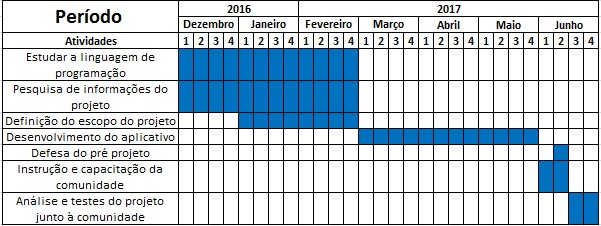
\includegraphics[width=1.0\linewidth]{imagens/cronograma_parte_1.jpg}
\end{figure}	

\begin{figure}[!h]
	\centering
	\caption{Cronograma parte 2}
	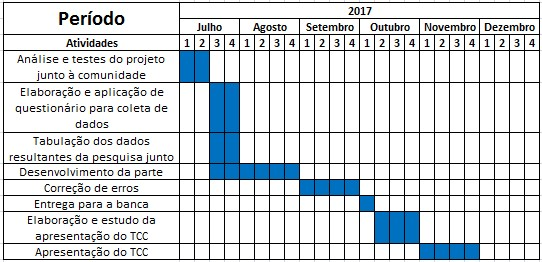
\includegraphics[width=1.0\linewidth]{imagens/cronograma_parte_2.jpg}
\end{figure}	


\chapter[Revisão Literária]{Revisão Literária}


O capítulo de revisão literária está dividido em 2 partes, sendo elas: ouvidoria e crowdsourcing.

\section{Ouvidoria}

\cite{cardoso2010ouvidoria} diz que a ouvidoria pública é o local para ser realizada a comunicação entre o cidadão e o Estado, onde eles possam agir em parceria e realizar um trabalho recíproco. 

Segundo \cite{assis2012ouvidoria}, a ouvidoria trabalha com a ideia que os usuários dos serviços prestados por algum órgão público ou privado eventualmente ficarão insatisfeitos com o serviço recebido e, em algum momento irão fazer alguma forma de protesto, seja ela uma reclamação, uma crítica, um pedido de reparação do serviço ou, em algumas ocasiões, se sentirão satisfeitos o bastante para elogiar o serviço. 

Tendo isso em mente, é possível entender que a ouvidoria é o órgão que vai realizar uma ponte de comunicação entre a prefeitura e os cidadãos, pois é capaz de “ouvir” as necessidades dos mesmos, e procurar atender de forma sensata suas necessidades.

Segundo \cite{assis2012ouvidoria}, as ouvidorias públicas se tornaram obrigatórias a todos os órgãos públicos que prestam algum tipo de serviço ao cidadão. Isso contribui para uma redução na qualidade das ouvidorias, pois em alguns órgãos não foram criadas por livre e espontânea vontade.

Segundo \cite{cardoso2010ouvidoria}, o ouvidor público deve ser ético, capaz de gerir e ter um conhecimento jurídico e social a respeito de uma cidade.

\section{Crowdsourcing}

Para \cite{decrowdbus}, crowdsourcing não possui uma tradução literal para o português, mas pode ser definido como Colaboração em Massa.

\cite{quirino2016estrategias} define o crowdsourcing como uma forma de resolução de problemas com a ajuda de um grande número de pessoas. Em paralelo, \cite{brabham2008crowdsourcing} analisa o \textit{crowdsourcing} como uma linha distribuída à resolução de problemas.

No contexto de uma cidade, o crowdsourcing trabalha lado a lado da ouvidoria pública, pois é através da multidão que o ouvidor consegue adiantar o trabalho da identificação de problemas, e retribui aos cidadãos dando um prazo para a resolução do mesmo, quando possível.

Além de corrigir esses problemas para o bem estar do cidadão, a correção de tais problemas previne que possíveis acidentes futuros possam ocorrer. Conforme \cite{rocha2013youonalert}, o crowdsourcing pretende ajudar na redução de acidentes com vítimas e também na redução de gastos públicos ao apoio dessas vítimas.


%% ----------------------------------------------------------
%
%Este documento e seu código-fonte são exemplos de referência de uso da classe
%\textsf{abntex2} e do pacote \textsf{abntex2cite}. O documento 
%exemplifica a elaboração de trabalho acadêmico (tese, dissertação e outros do
%gênero) produzido conforme a ABNT NBR 14724:2011 \emph{Informação e documentação
%- Trabalhos acadêmicos - Apresentação}.
%
%A expressão ``Modelo Canônico'' é utilizada para indicar que \abnTeX\ não é
%modelo específico de nenhuma universidade ou instituição, mas que implementa tão
%somente os requisitos das normas da ABNT. Uma lista completa das normas
%observadas pelo \abnTeX\ é apresentada em \citeonline{abntex2classe}.
%
%Sinta-se convidado a participar do projeto \abnTeX! Acesse o site do projeto em
%\url{http://www.abntex.net.br/}. Também fique livre para conhecer,
%estudar, alterar e redistribuir o trabalho do \abnTeX, desde que os arquivos
%modificados tenham seus nomes alterados e que os créditos sejam dados aos
%autores originais, nos termos da ``The \LaTeX\ Project Public
%License''\footnote{\url{http://www.latex-project.org/lppl.txt}}.
%
%Encorajamos que sejam realizadas customizações específicas deste exemplo para
%universidades e outras instituições --- como capas, folha de aprovação, etc.
%Porém, recomendamos que ao invés de se alterar diretamente os arquivos do
%\abnTeX, distribua-se arquivos com as respectivas customizações.
%Isso permite que futuras versões do \abnTeX~não se tornem automaticamente
%incompatíveis com as customizações promovidas. Consulte
%\citeonline{abntex2-wiki-como-customizar} par mais informações.
%
%Este documento deve ser utilizado como complemento dos manuais do \abnTeX\ 
%\cite{abntex2classe,abntex2cite,abntex2cite-alf} e da classe \textsf{memoir}
%\cite{memoir}. 
%
%Esperamos, sinceramente, que o \abnTeX\ aprimore a qualidade do trabalho que
%você produzirá, de modo que o principal esforço seja concentrado no principal:
%na contribuição científica.
%
%Equipe \abnTeX 
%
%Lauro César Araujo
%
%% ----------------------------------------------------------
%% PARTE
%% ----------------------------------------------------------
%\part{Preparação da pesquisa}
%% ----------------------------------------------------------
%
%% ---
%% Capitulo com exemplos de comandos inseridos de arquivo externo 
%% ---
%\include{abntex2-modelo-include-comandos}
%% ---
%
%% ----------------------------------------------------------
%% PARTE
%% ----------------------------------------------------------
%\part{Referenciais teóricos}
%% ----------------------------------------------------------
%
%% ---
%% Capitulo de revisão de literatura
%% ---
%\chapter{Lorem ipsum dolor sit amet}
%% ---
%
%% ---
%\section{Aliquam vestibulum fringilla lorem}
%% ---
%
%\lipsum[1]
%
%\lipsum[2-3]
%
%% ----------------------------------------------------------
%% PARTE
%% ----------------------------------------------------------
%\part{Resultados}
%% ----------------------------------------------------------
%
%% ---
%% primeiro capitulo de Resultados
%% ---
%\chapter{Lectus lobortis condimentum}
%% ---
%
%% ---
%\section{Vestibulum ante ipsum primis in faucibus orci luctus et ultrices
%posuere cubilia Curae}
%% ---
%
%\lipsum[21-22]
%
%% ---
%% segundo capitulo de Resultados
%% ---
%\chapter{Nam sed tellus sit amet lectus urna ullamcorper tristique interdum
%elementum}
%% ---
%
%% ---
%\section{Pellentesque sit amet pede ac sem eleifend consectetuer}
%% ---
%
%\lipsum[24]
%
%% ----------------------------------------------------------
%% Finaliza a parte no bookmark do PDF
%% para que se inicie o bookmark na raiz
%% e adiciona espaço de parte no Sumário
%% ----------------------------------------------------------
%\phantompart
%
%% ---
%% Conclusão
%% ---
%\chapter{Conclusão}
%% ---
%
%\lipsum[31-33]
%
%% ----------------------------------------------------------
%% ELEMENTOS PÓS-TEXTUAIS
%% ----------------------------------------------------------
%\postextual
%% ----------------------------------------------------------
%
%% ----------------------------------------------------------
%% Referências bibliográficas
%% ----------------------------------------------------------
\bibliography{abntex2-modelo-trabalho-academico}

% ----------------------------------------------------------
% Glossário
% ----------------------------------------------------------
%
% Consulte o manual da classe abntex2 para orientações sobre o glossário.
%
%\glossary

% ----------------------------------------------------------
% Apêndices
% ----------------------------------------------------------

% ---
% Inicia os apêndices
%% ---
%\begin{apendicesenv}
%
%% Imprime uma página indicando o início dos apêndices
%\partapendices
%
%% ----------------------------------------------------------
%\chapter{Quisque libero justo}
%% ----------------------------------------------------------
%
%\lipsum[50]
%
%% ----------------------------------------------------------
%\chapter{Nullam elementum urna vel imperdiet sodales elit ipsum pharetra ligula
%ac pretium ante justo a nulla curabitur tristique arcu eu metus}
%% ----------------------------------------------------------
%\lipsum[55-57]
%
%\end{apendicesenv}
%% ---
%
%
%% ----------------------------------------------------------
%% Anexos
%% ----------------------------------------------------------
%
%% ---
%% Inicia os anexos
%% ---
%\begin{anexosenv}
%
%% Imprime uma página indicando o início dos anexos
%\partanexos
%
%% ---
%\chapter{Morbi ultrices rutrum lorem.}
%% ---
%\lipsum[30]
%
%% ---
%\chapter{Cras non urna sed feugiat cum sociis natoque penatibus et magnis dis
%parturient montes nascetur ridiculus mus}
%% ---
%
%\lipsum[31]
%
%% ---
%\chapter{Fusce facilisis lacinia dui}
%% ---
%
%\lipsum[32]
%
%\end{anexosenv}
%
%%---------------------------------------------------------------------
%% INDICE REMISSIVO
%%---------------------------------------------------------------------
%\phantompart
%\printindex
%%---------------------------------------------------------------------

\end{document}
